Dieser Abschnitt befasst sich mit der gewählten Methode der qualitativen Inhaltsanalyse Mayrings. Dabei werden die einzelnen Schritte der Methode näher betrachtet und in die zugrunde liegende Theorie eingeordnet. Dabei wird herausgestellt, warum die Methode gewählt wurde.

\subsection{Qualitative Inhaltsanalyse nach Mayring}

Zur Untersuchung der \emph{kommunikativen Usability von RWTH Online} wurde ein qualitativer Forschungsansatz, in Form einer Nutzerstudie mit anschließendem retrospektiven Interview, gewählt.
Die gewählte Methode folgt der qualitativen Inhaltsanalyse nach \citeauthor{mayring2010qualitative}. Die von \citeauthor{mayring2010qualitative} entwickelte Methodik soll die Studiendaten schrittweise, systematisch und theoriegeleitet analysieren. Kernelement der Methode ist das Bestimmen von Kategorien, in denen während der Studie gefallene Aussagen zusammengefasst werden. Kategorien helfen, \textquote{die Studie nachzuvollziehen und die Befunden einzuordnen} (\cite[36]{meyen2011qualitative}). Die Oberkategorien werden zuerst anhand von Theorie deduktiv abgeleitet und später anhand des gesammelten Materials induktiv erweitert und verfeinert (vgl. \cite[13]{mayring2010qualitative}).

\subsection*{Analyseschritte nach Mayring}

\citeauthor{mayring2010qualitative} gibt systematische Schritte vor, denen eine Analyse von qualitativem Forschungsmaterial folgen muss, sodass es auch im Nachhinein möglich ist, diese nachzuvollziehen und zu reproduzieren (vgl. \cite[54]{mayring2010qualitative}). Folgende Auswertungsschritte sieht die qualitative Inhaltsanalyse nach \citeauthor{mayring2010qualitative} vor:

\begin{enumerate}
  \item Festlegung des Materials
  \item Analyse der Entstehungssituation
  \item Formale Charakteristika
  \item Richtung der Analyse
  \item Theoretische Differenzierung der Fragestellung
  \item Bestimmung der Analysetechnik und Festlegung des konkreten Ablaufmodels
  \item Definition der Analyseeinheit
  \item Rücküberprüfung des Kategoriensystems
  \item Interpretation der Ergebnisse und Richtung der Hauptfragestellung
  \item Anwendung der inhaltsanalytischen Gütekriterien
  \item Ein kaltes Bier öffnen und sich freuen % TODO: Entfernen
\end{enumerate}

Einige dieser Schritte sollen im Folgenden näher beleuchtet werden.

\subsection{Bestimmung des Ausgangsmaterials}

Der folgende Abschnitt umfasst die ersten drei Schritte, \textquote{Festlegung des Materials}, \textquote{Analyse der Entstehungssituation} und die \textquote{formale Charakteristika des Ausgangsmaterials} der qualitativen Inhaltsanalyse Maryrings (\cite[47]{mayring2010qualitative}). Zunächst soll jedoch der Studienablauf vorgestellt werden:

\subsection*{Festlegung des Materials: Nutzerstudie mit anschließendem Interview}

Zur Datenerhebung wurde eine Nutzerstudie mit anschließendem retrospektiven Interview durchgeführt. Zu Beginn der Studie wurden die Probanden gebeten, einen Fragebogen (siehe Anhang S. \pageref{att:Screeningbogen}) mit grundlegenden demographischen Daten und Angaben zur Vorerfahrung mit Campus Management Systemen (CMS) sowie Fragen zum allgemeinen Technikumgang auszufüllen. 
Während der Studie hatten die Probanden anschließend jeweils das gleiche Set von Aufgaben, die es mit der Anweisung zur Spontankommentierung (vgl. \cite{wharton1994cognitive}) zu bearbeiten galt. Bei der Spontankommentierung spricht die Versuchsperson laut aus, was sie gerade denkt und welche Handlungsschritte sie mit welchem Ziel unternimmt.

Das Ziel der Nutzerstudie ist es, Aussagen über das Nutzerverhalten in den konkreten, durch die Aufgaben spezifizierten Situationen zu erhalten. Der Vorteil dieses Vorgehens ist es, dass bei entsprechender Auswahl der Aufgaben natürliche Interaktionssituationen entstehen, die untersucht werden können. Während die Versuchsperson die Aufgaben bearbeitet, nimmt der Versuchsleiter eine beobachtende Rolle ein und greift ausschließlich zu organisatorischen Zwecken, wie zum Beispiel dem Abbrechen einer Aufgabe, in den Versuch ein (vgl. \cite{sarodnick2006methoden,rohrer_2014}). 
Gegenüber einem Experteninterview hat die gewählte Methode den Vorteil, dass mehr Feedback aus dem heterogenen Nutzerkreis von RWTH Online gesammelt werden kann. Ferner stand eine vollständige Neuentwicklung des Frontends von RWTH Online -- die vermutlich einstimmig durch Experteninterviews empfohlen worden wäre -- nicht zur Debatte. Durch die Nutzerstudie ist es daher möglich, einen ergebnisoffenen und detaillierten Einblick in die Thematik und deren Einbettung in den Alltag der Befragten, mit aller Komplexität, zu erhalten (vgl. \cite{sarodnick2006methoden,dumas1999practical}).

Nach vollständiger Bearbeitung der Aufgaben wurde ein retrospektives Interview anhand eines zuvor erstellten Leitfadens aufgezeichnet. In dieser Studie wurde im Fragebogen bewusst Raum gelassen, um dem Interviewleiter die Möglichkeit zu geben, auf bestimmte Situationen der Nutzerstudie einzugehen (vgl. \cite[113]{flick1995qualitative}).
Leitfadengespräche werden eingesetzt, wenn, wie im Falle diesere Studie, kleinere und interessante Gruppen befragt werden sollen. Sie werden dabei vor allem explorativ verwendet (vgl. \cite[184]{winfried1999empirische}). Teilstandardisierte Interviewleitfäden haben den Vorteil, dass der Interviewleiter sehr flexibel auf das Gespräch eingehen kann. Da der Interviewleiter die Reihenfolge der Fragen und deren Wortlaut in einem bestimmten Rahmen variieren kann, ist er in der Lage, offen auf unvorhergesehene Wendungen des Gesprächsverlaufs einzugehen (vgl. \cite[113]{flick1995qualitative}). Bei der Untersuchung der \emph{kommunikativen Usability} \textsuperscript{\textregistered} entsteht dadurch ein umfänglicheres Bild der Wirklichkeit. Der Befragte kann dabei frei von seinen Erfahrungen und Gedanken erzählen, auch personenbezogene Perspektiven werden besser beleuchtet. Ein weiterer Vorteil ist es, dass Fragen, die während des Gespräches redundant geworden sind, von dem Interviewleiter ausgelassen werden können. Dies wirkt sich positiv auf die Natürlichkeit des Interaktionsflusses zwischen Interviewleiter und Befragtem aus (vgl. \cite[391]{schnell1999methoden}).

\subsection*{Festlegung des Materials: Aufgabenset und Interviewleitfaden}
Bei der Planung der Studie wurde aus der persönlichen Erfahrung der Studierenden des Seminars Funktionen von RWTH Online besprochen, die unter einem oder mehreren Gesichtspunkten kritische Anwendungsfälle abdecken. Gesichtspunkte waren die \textit{Häufigkeit der Nutzung}, die \textit{Auswirkung von Fehlern} und \textit{offensichtlich mangelnde Bedienbarkeit}, die mit dem Expertenwissen der Seminarteilnehmenden attestiert werden konnte.

Mittels dieser Heuristik wurden folgende Anwendungsfälle identifiziert und passende Aufgaben erstellt:

\begin{enumerate}
    \item Prüfen des Zahlungseingangs für den Semesterbeitrag
    \item Ermitteln der bisher erarbeiteten Credit Points
    \item Verschaffen eines Überblicks über das Lehrangebot des kommenden Semesters
    \item Feststellen von Terminüberschneidungen
    \item Anmelden von Lehrveranstaltungen
    \item Finden von zu Lehrveranstaltungen gehörigen Prüfungen
    \item Anmelden zu Prüfungen
    \item Anzeigen der Notenübersicht
\end{enumerate}

Zu jedem Anwendungsfall wurde eine Aufgabe formuliert, lediglich die Punkte (4) und (5), sowie (6) und (7) wurden in jeweils einer Aufgabe zusammengefasst. Den Aufgaben vorangestellt wurde ein Szenario, das die Versuchsperson für die simulierte Situation einstimmen und den Aufgaben einen natürlichen Kontext geben sollte. Insgesamt wurden Szenario und Aufgaben in einem lockeren Ton formuliert und gelegentlich humoristisch aufgelockert, um die Probanden von der Erhebungssituation abzulenken und den Versuch etwas weniger formell und damit realitätsnäher wirken zu lassen. Das Szenario sowie die vollständigen Aufgabentexte befinden sich im Drehbuch der Studie, siehe Anhang auf Seite \pageref{att:Drehbuch}.

Der Leitfaden für das retrospektive Interview fragt zunächst einige grundsätzliche Punkte ab, wie eine gegenüberstellende Bewertung von RWTH Online zum alten CMS Campus Office und um die Vergabe einer Schulnote für RWTH Online. Anschließend stellt der Interviewleiter Fragen zu Dingen, die im Test aufgefallen sind, um möglicherweise nur implizit aufgekommene Probleme zu explizieren. Ferner wird der Studienablauf evaluiert und einige Fragen spezifisch zu Aspekten von RWTH Online gestellt.

\subsection*{Deduktives Kategoriensystem}
In der Ausgangssituation der Analyse wurde das im Seminar vorgestellte Kategoriensystem von \citeauthor{wirtz2009age} mit folgenden Kategorien zu Grunde gelegt (vgl. \cite{wirtz2009age}):

% Ich bin sehr stolz auf diese Tabelle
\begin{table}[h]
\def\arraystretch{1.1}
\begin{tabularx}{\textwidth}{|X|X|X|X|X|}
\hline
\textbf{Konsistenz\-probleme} & \textbf{Terminologie\-probleme} & \textbf{Strukturelle Probleme}       & \textbf{Feedback\-probleme} & \textbf{Layout\-probleme}\\ 
\hline
Inkonsistente Terminologie & Allgemeines Benennungsproblem & Allgemeines Strukturierungsproblem &      Fehlendes Feedback & Schriftproblem \\ 
\hline
Inkonsistente Farbgebung & Referenz\-problem & Kategori\-sierungs\-problem & Nicht-wahrnehmbares       Feedback & Schlechte Farbwahl und ungünstige Kontraste \\ 
\hline
Inkonsistente Beschriftung & Polysemie & Zuordnungs\-problem & Falsches Feedback & Probleme von        Bedienelementen \\ 
\hline
Inkonsistente Bedienabläufe & Verwendung von Fach- oder Fremdwörtern &  & Nicht-informatives           Feedback & Ungünstige räumliche Positionierung \\ 
\hline
& & & & Gestörte Form-Funktions\-beziehung \\ 
\hline
\end{tabularx}
\end{table}

\subsection*{Festlegung des Materials: Die Stichprobe}
Die vier Personen, die an der Studie teilgenommen haben waren Studenten der RWTH Aachen University (im Folgenden RWTH) der Informatik im Alter von 23 und 24 Jahren. Von den Befragten war eine Person weiblich, die anderen männlich. Ein Teilnehmer studiert im Bachelor, die anderen befinden sich im Master. Die Teilnehmer studieren bereits seit drei bis sechs Jahren an der RWTH und befinden sich in ihrem zweiten bis sechsten Fachsemester. Im Durchschnitt gaben die Versuchspersonen an, mit RWTH Online und CMS generell eher erfahren zu sein. Ferner gaben sie an, dass Technologie einen großen bis sehr großen Stellenwert in ihrem Alltag einnimmt. Drei der Teilnehmer gaben an, am Tag vier bis sechs Stunden im World Wide Web zu verbringen, ein Teilnehmer sogar sieben bis neun Stunden. Weiterhin schätzten die Teilnehmer ihre Frustrationstoleranz bei technischen Problemen als mittelmäßig bis gering ein. Drei der Befragten nutzen Google Chrome als ihren Standardbrowser, einer gab Mozilla Firefox als Standardbrowser an. Nach der Selbstauskunft bezüglich Fragen zum Technikumgang mit einem Auszug der Items des KUT-Fragebogens (vgl. \citeauthor{beier2004kontrolluberzeugungen}) sind die Probanden als durchweg erfahrene und selbstbewusste Techniknutzer zu beschreiben (siehe dazu Abbildung \ref{fig:technikkontrolle}).

\begin{figure}[hbt!]
 \centering
 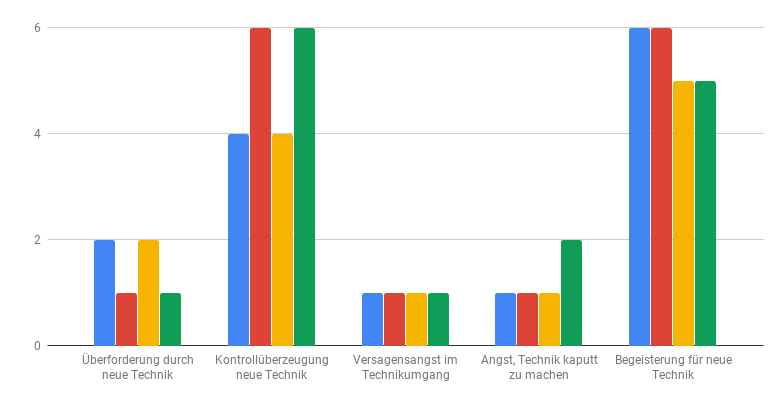
\includegraphics[width=\textwidth]{technikkontrolle.png}
 \caption{Selbsteinschätzung zur Technik-Kontrollüberzeugung mittels Auszug aus KUT (vgl. \cite{beier2004kontrolluberzeugungen}).}
 \label{fig:technikkontrolle}
\end{figure}

\subsubsection*{Analyse der Entstehungssituation}
Alle Probanden wurden über den erweiterten Bekanntenkreis der Seminarteilnehmer akquiriert. Um Erwünschtheitseffekte zu mindern wurde als Versuchsleiter in drei von den vier Studiendurchgängen ein Studierender festgelegt, der nicht zu dem Bekanntenkreis des Probanden gehört. Durchgeführt wurde die Erhebung in den Räumlichkeiten des Instituts für Sprach- und Kommunikationswissenschaft. Nach einer kurzen Begrüßung wurden die Kandidaten über den Studienablauf informiert, ihre Einverständnis zur Teilnahme und Datenerhebung sowie -auswertung eingeholt und der Screening-Fragebogen ausgefüllt. Vor dem Begin des Nutzertests wurden die Teilnehmer angewiesen, anhand von einem Überraschungsei die Spontankommentierung zu üben.

Erst danach wurden die Probanden zum bearbeiten der Aufgaben ein Laptop der Marke Lenovo/IBM bereitgestellt, der per WLAN an das Internet des Instituts angebunden war. Bereits für die Probanden vorbereitet war der Webbrowser Google Chrome mit geöffnetem RWTH Online. Dort wurden die Probanden in einen von ihren persönlichen Daten unabhängigen Nutzeraccount eingeloggt. Den Probanden wurde mitgeteilt, dass sie nicht auf dem tatsächlichen RWTH Online System arbeiten, sondern auf einem Klon. Für die Interaktion wurde den Teilnehmern freigestellt, das Trackpad oder die angeschlossene Maus zu nutzen. 

Nach Abschluss des Nutzertests wurden die Probanden im retrospektiven Interview in einem teilstandardisierten Leitfadengespräch zu dem Nutzertest und zu RWTH Online allgemein befragt. 

\subsubsection*{Formale Charakteristika des Ausgangsmaterials}
Alle vier Nutzerstudien wurden innerhalb eines Tages durchgeführt. Die Daten des Screening-Fragebogens liegen in Tabellenform digitalisiert vor, die Interaktion der Versuchspersonen während des Nutzertests wurde audiovisuell (Mimik, Audio und Screencapture) aufgezeichnet und nach GAT 2 transkribiert (vgl. \cite{selting1998gesprachsanalytisches}). Das retrospektive Interview wurde mit einem handelsüblichen Smartphone akustisch aufgezeichnet und ebenfalls transkribiert. Die transkribierten Dateien wurden anschließend kodiert. Zum Transkribieren und Kodieren wurde die Software MAXQDA eingesetzt. MAXQDA unterstützt die qualitative Inhaltsanalyse bei der Organisation und Visualisierung der Kodierung und des Kategoriensystems.

\subsection{Fragestellung der Analyse}
Nach Mayring setzt sich der nächste Schritt, die \textquote{Fragestellung der Analyse} aus der \textquote{Richtung der Analyse} und der \textquote{Theoretischen Differenzierung der Fragestellung} zusammen \cite[53]{mayring2010qualitative}). Innerhalb dieser Schritte wird der Gegenstand der Untersuchung und die Forschungsfrage klarifiziert.

Die Nutzerstudie untersucht das CMS RWTH Online daraufhin, welche Aspekte der kommunikativen Usability verbessert werden können. Dabei wurden zufällig ausgewählte Personen der Zielgruppe \textit{Student der Informatik} befragt.

\subsection{Datenanalysetechnik und Analyseeinheit}
Vor der eigentlichen Methodenanwendung muss die \textquote{Bestimmung der Analysetechnik} und die \textquote{Definition der Analyseeinheit} vollzogen werden. Unter Analysetechnik versteht \citeauthor{mayring2010qualitative} drei Techniken, anhand deren das Datenmaterial analysiert wird.

In dieser Studie wurden vor allem die Analysetechnik \textquote{Zusammenfassung} und \textquote{Explikation} genutzt. Das bedeutet, dass zuerst das Datenmaterial auf die wesentlichen Inhalten reduziert wird, beispielsweise durch die Reduktion von redundanten Textpassagen und anschließend, unter Einbezug des Kontext unter denen die Aussagen entstanden sind, erklärt werden. Während das \textquote{Abbild des Grundmaterials} erhalten bleibt, wird der Korpus übersichtlicher (vgl. \cite[115]{mayring2010qualitative}). Die größte Analyseeinheit bestand in Passagen, die kleinste in einzelnen Worten.

\subsection{Methodenanwendung}
In der eigentlichen Methodenanwendung werden die oben angesprochenen Kategorien gebildet. Dies kann deduktiv, anhand der vorhergegangenen theoretischen Überlegungen oder induktiv, anhand des gesammelten Materials, geschehen. Anschließend werden die gebildeten Kategorien anhand eines Ankerbeispiels aus dem Material festgemacht.

Insgesamt sind \emph{TODO: ZAHL EINFÜGEN} Analyseeinheiten aus den Nutzertests und Interviews extrahiert worden und bilden den Korpus des Kategoriensystems. Die gesammelten Daten sind analysiert und den passenden Kategorien zugeordnet worden. Falls ein Datum nicht in eine bestehende Kategorie passten, wurde induktiv eine weiter Kategorie gebildet. War es möglich mehrere Daten unter einer Unterkategorie zusammenfassen, wurde auch diese Kategorie induktiv aus dem Material gebildet und einer bestehenden Oberkategorie zugeordnet. In weiteren Analyseiterationen wurde geprüft, ob sich die einzelen Daten überscheidungsfrei den Kategorien zuordnen lassen. Eine beispielhafte Oberkategorie mit Unterkategorie und entsprechenden Ankerbeispiel sieht wie folgt aus:

\emph{TODO: BEISPIEL EINFÜGEN}

Das finale Kategoriensystem umfasste die Oberkategorien \emph{TODO: KATEGORIEN EINFÜGEN}. Die Bedeutung der einzelnen Kategorien lässt sich gut an der Namensgebung ablesen. Weitere Unterkategorien sind induktiv aus dem Datenmaterial erschlossen worden und werden im Ergebnissteil genauer beleuchtet. Das finale System aus Oberkategorien sieht wie folgt aus:

\emph{TODO: BILD DER OBERKATEGORIEN EINFÜGEN}